% Created with jtex v.1.0.1
\documentclass[twocolumn, switch]{article}
\usepackage{preprint}
\usepackage{hyperref}
\usepackage[numbers,square]{natbib}

%%%%%%%%%%%%%%%%%%%%%%%%%%%%%%%%%%%%%%%%%%%%%%%%%%
%%%%%%%%%%%%%%%%%%%%  imports  %%%%%%%%%%%%%%%%%%%
\usepackage{graphicx}
%%%%%%%%%%%%%%%%%%%%%%%%%%%%%%%%%%%%%%%%%%%%%%%%%%

% colors for hyperlinks
\hypersetup{colorlinks=true, linkcolor=purple, urlcolor=blue, citecolor=cyan, anchorcolor=black}

\usepackage[utf8]{inputenc}	% allow utf-8 input
\usepackage[T1]{fontenc}
\usepackage{xcolor}
\usepackage{lineno}					% Line numbers
\usepackage{tikz} 					% ORCiD insertion

%% Bibliography options
\bibliographystyle{unsrtnat}

 %% Special figure caption options
\usepackage{newfloat}
\DeclareFloatingEnvironment[name={Supplementary Figure}]{suppfigure}
\usepackage{sidecap}
\sidecaptionvpos{figure}{c}

% Section title spacing  options
\usepackage{titlesec}
\titlespacing\section{0pt}{12pt plus 3pt minus 3pt}{1pt plus 1pt minus 1pt}
\titlespacing\subsection{0pt}{10pt plus 3pt minus 3pt}{1pt plus 1pt minus 1pt}
\titlespacing\subsubsection{0pt}{8pt plus 3pt minus 3pt}{1pt plus 1pt minus 1pt}

\definecolor{lime}{HTML}{A6CE39}
\DeclareRobustCommand{\orcidicon}{
	
\begin{tikzpicture}
	\draw[lime, fill=lime] (0,0)
	circle [radius=0.16]
	node[white] {{\fontfamily{qag}\selectfont \tiny ID}};
	\draw[white, fill=white] (-0.0625,0.095)
	circle [radius=0.007];
	\end{tikzpicture}
	\hspace{-2mm}
}

%%%%%%%%%%%%%%%%   Title   %%%%%%%%%%%%%%%%
\title{The attractor states of the functional brain connectome}

% Add watermark with submission status
% Awaiting watermark support
% \usepackage{xwatermark}
% % Left watermark
% \newwatermark[firstpage,color=gray!60,angle=90,scale=0.32, xpos=-4.05in,ypos=0]{\href{https://doi.org/}{\color{gray}{Publication doi}}}
% % Right watermark
% \newwatermark[firstpage,color=gray!60,angle=90,scale=0.32, xpos=3.9in,ypos=0]{\href{https://doi.org/}{\color{gray}{Preprint doi}}}
% % Bottom watermark
% \newwatermark[firstpage,color=gray!90,angle=0,scale=0.28, xpos=0in,ypos=-5in]{*correspondence: \texttt{}}

%%%%%%%%%%%%%%%  Author list  %%%%%%%%%%%%%%%
\usepackage{authblk}
\renewcommand*{\Authfont}{\bfseries}

\author[1\thanks{\texttt{robert.englert@uk-essen.de}}]{Robert Englert}
\author[1\thanks{\texttt{tamas.spisak@uk-essen.de}}]{Tamas Spisak}
\affil[1]{University Medicine Essen}

%%%%%%%%%%%%%%    Front matter    %%%%%%%%%%%%%%
\begin{document}

\twocolumn[\begin{@twocolumnfalse}

\maketitle

\begin{abstract}
Todo\\
\end{abstract}

\keywords{}

\vspace{0.5cm}

\end{@twocolumnfalse}]

%%%%%%%%%%%%%%%  Main text   %%%%%%%%%%%%%%%

\textbf{Highglights:}

\begin{itemize}
\item a
\item b
\end{itemize}

\subsection{Introduction}\label{Introduction}

Functional brain connectomics studies the spontaneous co-activation of brain regions and has revolutionized our understanding of the physical basis of mind [ref]. The majority of fMRI connectivity studies assume temporal stationarity, i.e. that the brain connectivity is static for the entire data acquisition period. Such studies have provided a wealth of insights into the neural mechanisms of several behavioral/psychological phenotypes and clinical conditions. However, functional connectivity has been shown to be dynamic; it fluctuates spontaneously over time in a globally coordinated manner. Dynamic functional connectivity has quasi periodic properties (ref), with a limited number of recurring states (``brain states'') \cite{Gutierrez_Barragan_2019}; i.e. sporadic intervals during which information can be efficiently exchanged between a characteristic subset of brain regions [Hutchison et al., 2013, Liu 2013 PNAS, Zalesky, PNAS, 2014]. Brain state dynamics can be assessed with multiple techniques, including independent component analysis (ref), co-activation patterns (Liu 2013 PNAS), \dots and there is accumulating evidence for the neurobiological relevance of these dynamics, with promising perspectives for facilitating the clinical translation of functional neuroimaging techniques by improving brain based biomarkers (Woo, Nat Med. 2021).

However, progress is limited by gaps in the mechanistic understanding of how brain activity and functional connectivity dynamically shape each other and how this process leads to the emergence and organization of brain states (ref).

Here we propose a novel model-based framework that - with minimal, but reasonable assumptions about the ``activity flow'' (ref: Cole-papers) between two, functionally connected regions - considers the stationary functional brain network as an empirical (i.e. already-trained) artificial neural network (eANN). In the proposed framework, the topology of the stationary brain connectome defines a cost (energy) for any arbitrary brain activation patterns and a trajectory towards one of the finite number of stable patterns that minimize this cost (so-called attractor states).

Here we propose these attractors states as robust and biomedically relevant characteristics of the functional brain connectome, with a wide variety of potential applications.

We demonstrate that the proposed attractor states highly resemble to the dynamic brain states commonly observed by dynamic functional connectivity methods (e.g. CAP-analyses (ref)) and provide a proof-of-concept for the biomedical validity of our framework, by showing that the average brain activations corresponding to the attractor states during resting sate display manifold significant associations to cognition.

Due to the known noise-tolerance of the applied eANN-s, the proposed approach can be expected to be highly robust/reliable/replicable, which we demonstrate with independent datasets (total n=xxx).

List all the aims: hierarchy, generalizability etc

\subsection{Results}\label{Results}

\begin{figure}[!htbp]
\centering
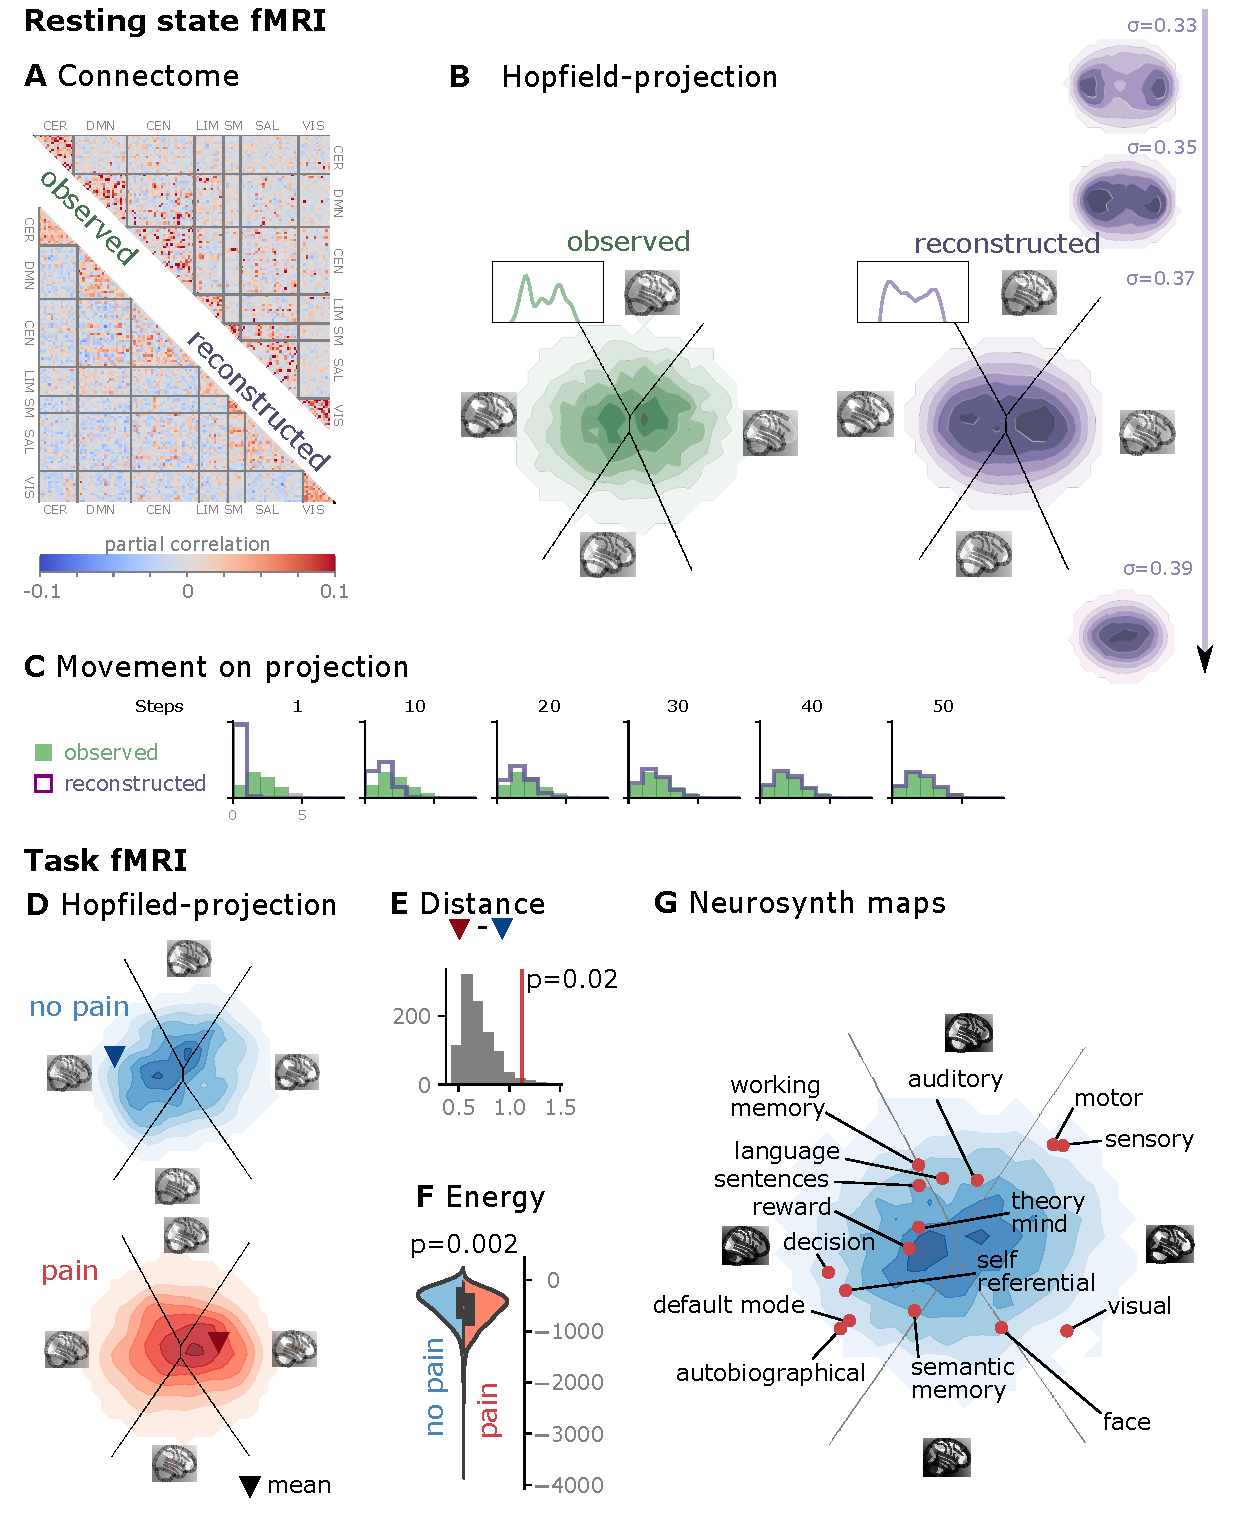
\includegraphics[width=0.7\linewidth]{files/face_validity-4e24c8a7fab5d067b4dc83e1cb6229f1.pdf}
\caption{Empirical Hopfiled-networks reconstruct real brain activity.}
\label{Figure 1}
\end{figure}

\subsection{Discussion}\label{Discussion}

\subsection{Methods}\label{Methods}

Todo

Todo



%%%%%%%%%%%%%%   Bibliography   %%%%%%%%%%%%%%
\bibliography{main.bib}

\end{document}
